\section{Creep}

Creep is a time-dependent and/or temperature-dependent deformation
process of a solid body under the influence of a constant load.
%
Creep is a phenomenon of time effect to deformation such that the
tendency of a material to move or to deform is permanent to relieve
stresses. Similar to plastic potential, a creep potential $F_c$ is
introduced to describe the constitutive equations.

Usually, a stationary creep model is sufficient to describe the
creep phenomena in geological media, such as soil and rock. Norton's
model reads that the creep potential $F_c$ can be expressed by a
function of the first stress invariant $\sivi$ as
%
\begin{equation}
F_c = \frac{\alpha}{n+1}\,\sivi^{n+1}
\end{equation}
%
where $\alpha$ and $n$ are material parameters, which have to be
determined by experiments.
%
Assuming the total strain increment $d \Stra$ is admissible to be
decomposed in several portions contributed by different physical
reactions such elasticity, plasticity and creep, it can be written
as
%
\begin{equation}
d \Stra = d \Stra^{e}+d \Stra^{p}+d \Stra^{c}
\end{equation}
%
Similar to the plastic flow rule, we can derive the strain rate
resulting from creep as
%
\begin{equation}
d \Stra^{c}
=
\frac{ \partial F_c}{\partial \Stress}
=
\left(\frac{3}{2}\right)^{(n+1)/2}
\alpha\left\Vert {\devS}
\right\Vert^{n-1}\devS
\label{eq:crpflow}
\end{equation}

Applying explicit Euler's method to equation (\ref{eq:crpflow}), the
increment of the strain by creep is obtained from
%
\begin{equation}
\Delta \Stra^{c}  =
\left(\frac{3}{2}\right)^{\frac{n+1}{2}}\alpha\norm{\devS^k}^{n-1}\devS^k
\Delta t \label{eq:dstrain_crp}
\end{equation}
%
where $\devS^k$ is the deviatoric stress of the previous time step
$k$ and $ \Delta t$ is the time step size.
%
Using the generalized Hook's law, the stress change deduced by the
creep stain increment is
%
\begin{equation}
\Delta \Stress^{c}  =  \mathbf D^{e} \Delta \Stra^{c}
\label{eq:dstress_crp}
\end{equation}
%
with $\mathbf D^{e}$ the elastic material tensor.


\subsection{Creep of a cylindrical sample}

\subsubsection*{Problem definition}

In this example, creep is considered in a thick cylinder subjected a
constant normal pressure at the inner face.
%
The boundary conditions are as follows: $p$ =2.515 MPa at the inner
surface and zero normal stress at the outer surface, no
displacements in axial direction. The inner radius of the
cylindrical sample is 4 mm, the outer radius is 6.4 mm and the
height is 1 mm. Quadrilateral elements are adopted for meshing (Fig.
\ref{fig:meshcrp}).
%
\begin{figure}[!htb]
\centering
\includegraphics[scale=0.3]{M/mesh_crp}
\caption{Mesh for thick cylinder undergos creep deformation}
\label{fig:meshcrp}
\end{figure}

We assume that the initial stress is homogeneously distributed in
the domain as $\sigma_{r}^0=\sigma_{\theta}^0=\sigma_{z}^0=-50$ Pa.
The parameters of the Norton creep model are given in Tab.
\ref{tab:creep_norton}.

\begin{table}[H]
\center
\begin{tabular}{llrl}
\hline\noalign{\smallskip}
\hline
Symbol & Meaning & Value & Unit \\
\hline
$\alpha$ & Norton model parameter 1 & $6.415\times 10^{-10}$ & -- \\
$n$      & Norton model parameter 2 & $4$ & -- \\
$\nu$    & Poisson ratio & $0.48$ & -- \\
$E$      & Young's modulus & $1.378\times10^5$ & MPa \\
\hline\hline
\end{tabular}
\caption{Material parameters of the Norton creep model} %\footnotesize
\label{tab:creep_norton}
\end{table}


\subsubsection*{Results}

Figs. \ref{fig:ex2_q} and \ref{fig:ex2_ur} give the distribution of
the first stress invariant and radial displacement along radial
direction and the comparison with pure elastic solution. They
demonstrated that $\mathbf s$ at inner surface decreases about 26\%
after steady state of creep reached. While radial displacements
increase about 200\%.
%
The results can be compared with Balley's analytical solution, which
reads for rate of radial displacement as
%
\[
  \dot u_{r} =\alpha \dfrac{3^{\frac{n+1}{2}}}{2n^n}\dfrac{r_{a}^2\;r_{b}^2\;p^n}{(r_{b}^{2/n}-r_{a}^{2/n})r}
%% \label{eq:balleyu}
\]
and for the steady state of first stress invariant
\[
  \sigma_v =\dfrac{2\sqrt 3}{2n} \dfrac{p\;\left(r_b/r\right)^{\frac{2}{n}}}{(r_{b}/r_a)^{2/n}-1}
%% \label{eq:balleys}
\]

\subsubsection*{Benchmark deposit}
\begin{tabular}{|l|l|l|}
  \hline
  Benchmark & Problem type & Path in benchmark deposit \\
  \hline
 \emph{m\_crp\_tri}& M & benchmarks\verb \M\ \\
  \hline
\end{tabular}

\begin{figure}[H]
\centering
\includegraphics[scale=0.4]{M/crp/ex2_q}
\vspace{-3mm}
\caption{First stress invariant profiles during creep at different times, $t$ = 5,25,50 sec,
and comparison to elastic solution}
\label{fig:ex2_q}
\end{figure}

\begin{figure}[H]
\centering
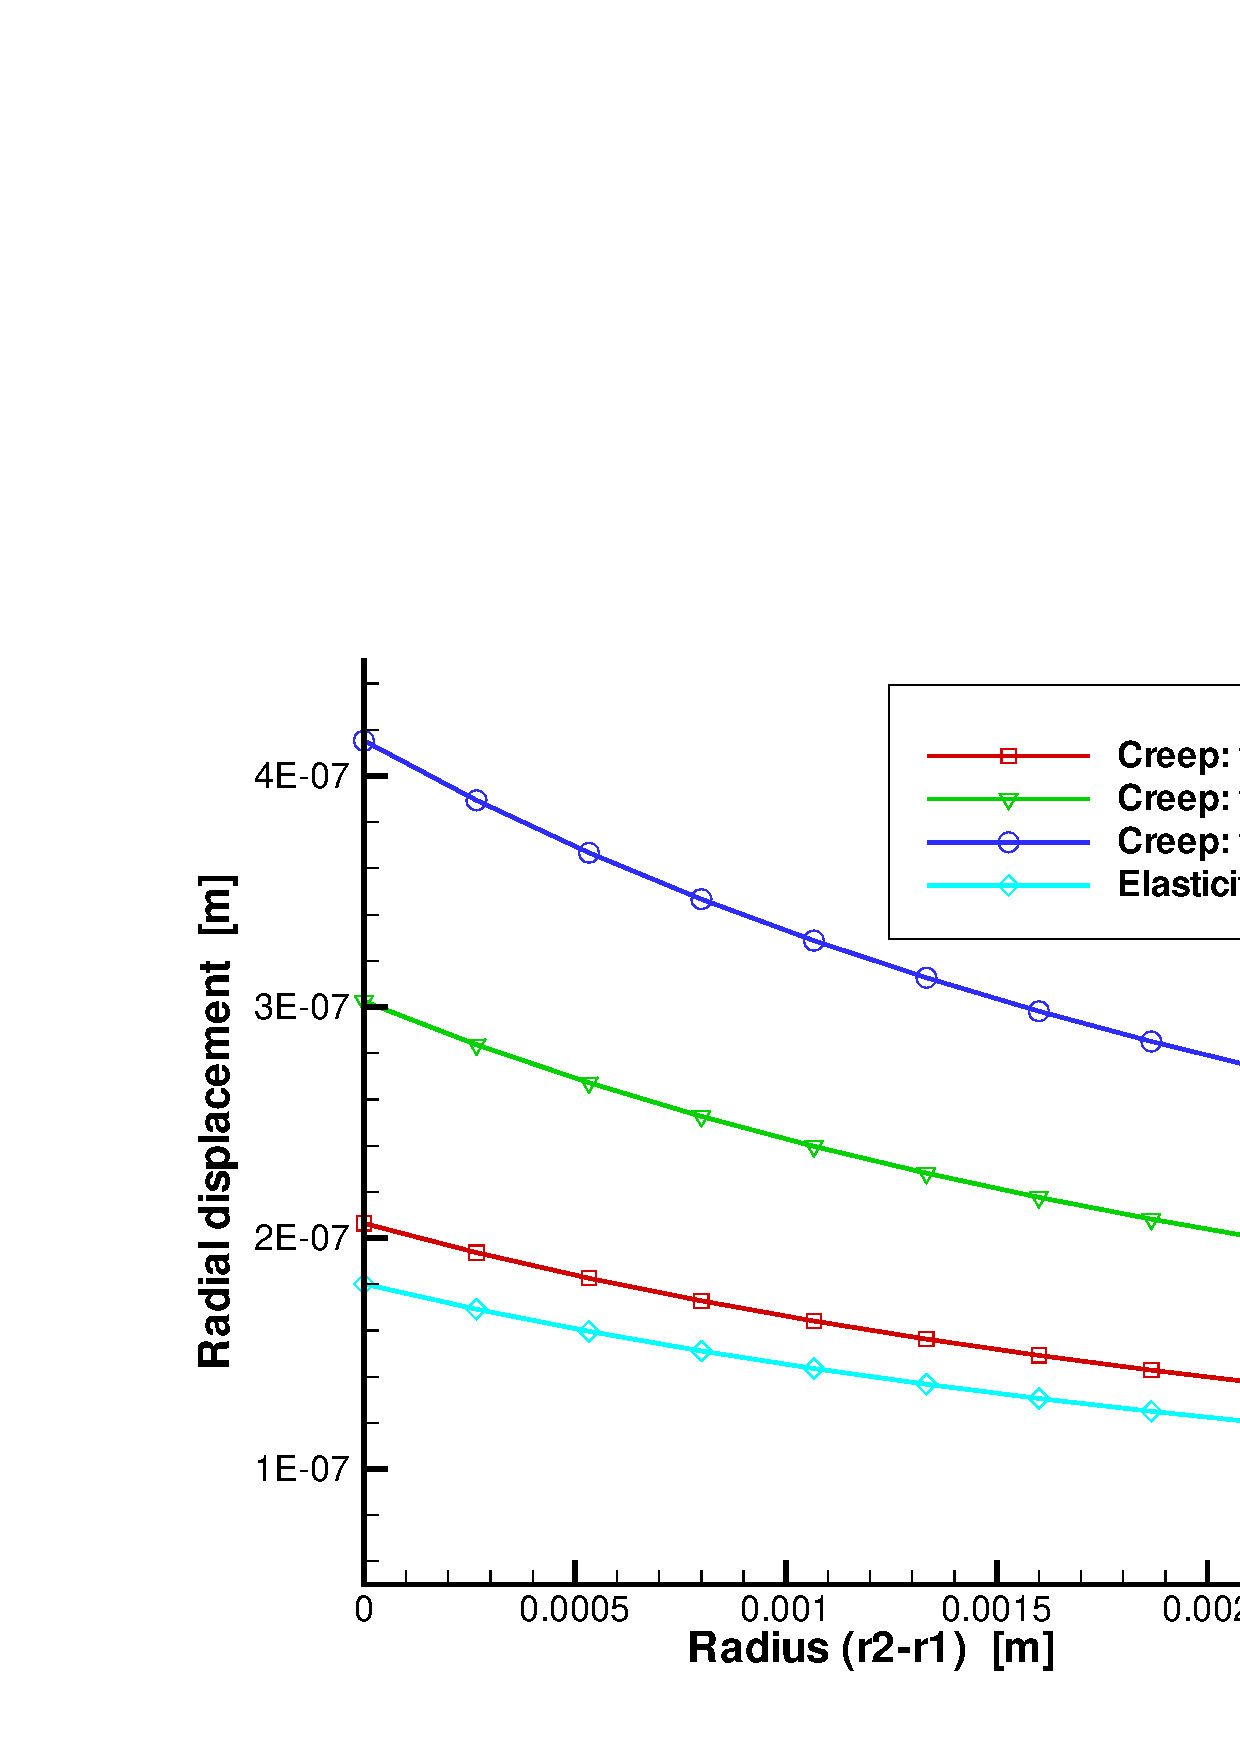
\includegraphics[scale=0.4]{M/crp/ex2_ur}
\vspace{-3mm}
\caption{Radial displacement profiles during creep at different times, $t$ = 5,25,50 sec,
and comparison to elastic solution}
\label{fig:ex2_ur}
\end{figure}
